% --------------------------------------------------------------
% This is all preamble stuff that you don't have to worry about.
% Head down to where it says "Start here"
% --------------------------------------------------------------

\documentclass[12pt]{article}

\usepackage[margin=0.8in]{geometry}
\usepackage{amsmath,amsthm,amssymb}
\usepackage{multicol}
\usepackage{graphicx}
\usepackage{fixltx2e}
\usepackage{amsmath}

\usepackage{tikz}
\usepackage{pgfplots}
\usepackage{fourier}

\newcommand{\N}{\mathbb{N}}
\newcommand{\Z}{\mathbb{Z}}

\begin{document}

% --------------------------------------------------------------
%                         Start here
% --------------------------------------------------------------

%\renewcommand{\qedsymbol}{\filledbox}

\title{Tutorial III}%replace X with the appropriate number
\author{EN1060 - Signals and Systems\\} %if necessary, replace with your course title

\maketitle
\begin{enumerate}
\item Find following convolutions:
\begin{enumerate}
    \item $x(t)\ast\delta(t)$
    \item $x(t)\ast\delta(t-t_0)$
    \item $x(t)\ast u(t)$
    \item $x(t)\ast u(t-t_0)$
\end{enumerate}

\item Let $y(t) = x(t)\ast h(t)$. Show that $x(t-t_1)\ast h(t-t_2) = y(t-t_1-t_2)$

\item Find $y(t)$ of the following system and signal.

\begin{figure}[h]
    \centering
    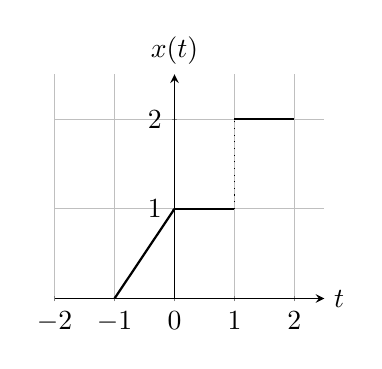
\begin{tikzpicture}
	\begin{axis}[
		xscale = 0.5,
		yscale = 0.5,
		xmin= -2, xmax = 2.5,
		ymin= 0, ymax = 2.5,
		axis x line=bottom,
		axis y line=center,
		xtick = {-2,-1,0,1,2, 3},
		ytick = {1, 2},
		xlabel=$t$, xlabel style={at={(ticklabel* cs:1)}, anchor= west},
		ylabel=$x(t)$, ylabel style={at={(ticklabel* cs:1)}, anchor=south},
		grid=both,
		]
		\addplot[domain=-1:0, thick] (\x, \x+1);
		\addplot[domain=0:1, thick] (\x, 1);
        \addplot[domain=1:2, thick] (\x, 2);
		\draw[dotted] (axis cs:1,1) -- (axis cs:1,2);
        \end{axis}
\end{tikzpicture}
\caption{}
\end{figure}

\item Compute and sketch $y[n] = x[n]\ast h[n]$ for the following:

\begin{enumerate}
    \item $ x[n] = \alpha^{n}u[n]$ \hspace{1cm} and \hspace{1cm} $h[n] = \beta^{n}u[n] , \alpha < \beta$
    \item $x[n] = \alpha^{n}u[n]$  \hspace{1cm} and \hspace{1cm} $h[n] = \alpha^{-n}u[-n]$
\end{enumerate}

\item Consider the continuous time LTI system whose step response is $s(t) = e^{-t}u(t)$. Determine the output of following $x(t)$. 

\begin{figure}[h]
    \centering
    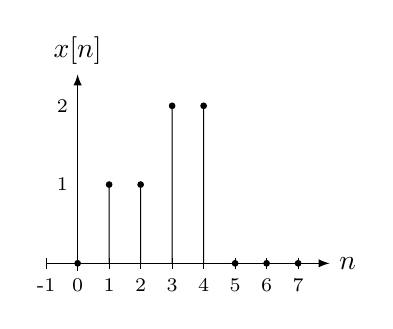
\begin{tikzpicture}
    \draw[-latex] (-1*0.4,0) -- (8*0.4,0) node[anchor=west] {$n$};
    \draw[-latex] (0, -0.1) -- ++(0,2.5) node[anchor=south] {$x[n]$};
    \foreach \x in {0}
        {
            \draw[fill=black] (\x*0.4, 0) circle (1pt);
        }
    \foreach \x in {1,2}
        {
            \draw[fill=black] (\x*0.4, 0)  -- ++(0,1) circle (1pt);
        }
    \foreach \x in {3,4}
        {
            \draw[fill=black] (\x*0.4, 0)  -- ++(0,2) circle (1pt);
        }        
        
    \foreach \x in {5,6,7}
        {
            \draw[fill=black] (\x*0.4, 0) circle (1pt);
        }        
    \foreach \x in {-1, 0, ..., 7}
    {
        \draw (\x*0.4, 2pt) -- ++(0, -4pt) node[anchor=north]{\scriptsize \x};
    }
    \foreach \y in {1,2}
    {    
    	\node at (0,\y) [anchor=east] {\scriptsize \y};
    }
\end{tikzpicture} 
\caption{}
\end{figure}

\item A system is formed by connecting two systems in cascade. The impulse response of those systems are given by $h_{1}(t)$ and $h_{2}(t)$ where,  
     \begin{align*}
        h_1(t) &= e^{-2t}u(t)&\hspace{2cm} h_2(t) &= 2e^{-t}u(t)
     \end{align*}
\begin{enumerate}
    \item Find the impulse response of the overall system.
    \item Determine whether the overall system is BIBO stable.
\end{enumerate}

\item Show that if the input $x[n]$ to a discrete time LTI system is periodic with period $N$, then the output $y[n]$ is also periodic with period $N$.

\item Consider a discrete time system $S_1$ with $h[n] = (1/5)^{n}u[n]$.

\begin{enumerate}
    \item Find the integer $A$ such that $ h[n] - Ah[n] = \delta[n] $
    \item Using the result from part (a) determine the impulse response $g[n]$ of the LTI system $S_2$, which is the inverse of system $S_1$.
\end{enumerate}

\item Let $x(t) = 1 + \sin(\omega_0t) + 2cos(\omega_0t) + \cos(2\omega_0t)+\pi/4)$ which has fundamental frequency $\omega_0$ Give this as a linear combination of complex exponentials and identify Fourier series coefficients.
    
\item Consider the convolution
        \begin{equation*}
            y(t) = \sin(\pi t) \left[u(t+1) - u(t-1)\right] \ast \left[u(t+1) - u(t-1)\right]
        \end{equation*}
        \begin{enumerate}
            \item Sketch the two signals.
            \item Evaluate the convolution.
        \end{enumerate}
    

\end{enumerate}

% --------------------------------------------------------------
%     You don't have to mess with anything below this line.
% --------------------------------------------------------------

\end{document} 